\justifying

%%%%%%%%%%%%%%%%%%%%%%%%%%%%%%%%%%%%%%%%%%%%%%%%
\section{Introduction} \label{sec:intro}
%%%%%%%%%%%%%%%%%%%%%%%%%%%%%%%%%%%%%%%%%%%%%%%%

The remarkable technological progress attained in the last few decades has yielded significant benefits in the form of highly advanced imaging, spectroscopic, and polarimetric instruments designed for astronomical observations. These instruments have empowered us with the ability to scrutinize the Sun with exceptional detail. While some of these are ground based telescopes, the others operate from space. Primarily, space-based instruments observe the Sun in Ultraviolet (UV), extreme ultraviolet (EUV), and X-ray bands, capturing radiation from upper atmospheric layers such as the transition region and corona
, which emit due to their elevated temperatures. Various studies of the Sun over the last few decades have successfully uncovered the physical properties of the gas in the upper layers of the solar atmosphere using the observations recorded by X-ray imaging ({\it Hinode} X-ray Telescope \citep[{\it Hindoe}/XRT,][]{xrt}) and spectroscopy (the Spectrometer/Telescope for Imaging X-rays on {\it Solar Orbiter} \citep[{\it SO}/STIX,][]{stix}) and extreme ultraviolet (EUV) imaging (Atmospheric Imaging Assembly on the {\it Solar Dynamic Observatory} \cite[{\it SDO}/AIA,][]{aia}, Extreme ultraviolet Imaging Telescope on {\it Solar and Heliospheric Observatory} \cite[{\it SoHO}/EIT,][]{eit}, Solar Ultraviolet Imager on the {\it Geostationary Operational Environmental Satellites} \citep[{\it GOES}/SUVI,][]{suvi}, the Extreme Ultraviolet Imager on {\it Solar Terrestrial Relations Observatory-A} \cite[{\it STEREO-A}/EUVI,][]{stereo,euvi}, \textbf{the Extreme-Ultraviolet Imager on {\it SO} \citep[{\it SO}/EUI][]{eui}}) and spectroscopy \citep[Hinode/EIS,][]{eis}, among many others. The {\it Transition Region and Coronal Explorer} \citep[{\it TRACE},][]{trace}, \textbf{the Solar Ultraviolet Measurements of Emitted Radiation on {\it SoHO} \citep[{\it SoHO}/SUMER,][]{sumer}} and the {\it Interface Region Imaging Spectrograph} \citep[~{\it IRIS},][]{iris} allowed us to probe the chromosphere and the transition region in detail. These missions provide us with continuous full disk and Region of Interest (RoI) coverage of the Sun over the X-ray and EUV wavelengths. The situation is rather different in the Near-Ultraviolet (NUV) regime. There is clearly a lack of continuous coverage of the full solar disk in this wavelength range. 

One of the key challenges of carrying out Solar observations in the UV regime from ground is the strong attenuation by the Earth's atmosphere. To circumnavigate this, one of the first stratospheric balloon-borne instrument was flown in 1970 and 1971 by \cite{herse79}. The instrument carried a 20 cm telescope that imaged the sun in 200{--}460 nm. The Rasolba balloon experiment was composed of a 30 cm telescope with an ultraviolet spectrograph. They obtained high resolution spectra of the Sun in the spectral range 190 {--} 295 nm \citep{samain85,staath95}. Sunrise \citep{sunrise1,sunrise2} is a balloon-borne observatory that followed up these instruments to observe the Sun in the Near UltraViolet (NUV) regime with a telescope of 1 m diameter. It has flown twice, in June 2009 and June 2013, respectively and provided us with high resolution imaging in 214, 300, 312, 388 and 397~nm with the Sunrise Filter Imager \citep[SuFI,][]{sufi} in 2009 and at 214, 279 and 397~nm in 2017 \citep{sunrise2}, Dopplergrams and vector magnetorams in \ion{Fe}{1} 525.02 nm with the Imaging Magnetograph eXperiment \citep[IMaX,][]{imax} at various locations on the Solar disk.  During these two flights, along with quiet sun and active regions, Sunrise observed various solar phenomenon e.g. emerging flux events \citep{centeno17}, properties and dynamics of moving magnetic features around pores \citep{kaithakkal17}, proper motion of bright points in quiet sun and active regions \citep{jafarzadeh17}, properites of fibrils \citep{gaferia17} etc. These observations demonstrated the wealth of information this wavelength range carries and opened the path for full disk coverage of the Sun in the NUV. 


The Solar Ultraviolet Imaging Telescope \citep[SUIT;][]{ghosh16,article} is one of the seven payloads onboard the Aditya-L1 mission \citep{adityal1, aditya} of the Indian Space Research Organization (ISRO), launched on September 2, 2023. The satellite is placed in a halo orbit around the Sun-Earth L1 point. With its eleven science filters (eight narrow band and three broad band), {\suit} has the unique capability to probe different heights in the solar photosphere and chromosphere; helping us to understand various physical processes responsible for the transport of mass and energy from one layer to another. Moreover, SUIT provides the unique opportunity to measure the spatially resolved solar spectral irradiance in the NUV, which is central to our understanding of Sun climate relations. 

{\suit} is designed to provide full-disk and RoI images of the Sun continuously, with a plate scale of 0.7{\arcsec}. It has the capability of tracking the RoIs while compensating for the differential rotation \citep{suit_algo}. Moreover, it is also capable of detecting and localizing flares with on-board intelligence and can also automatically control the exposure time to avoid saturation. The main science questions that {\suit} aims to address are \citep[][]{suit_science,suit_main}: 

\begin{itemize}
    \item Coupling and dynamics of the solar atmosphere: {\it How is energy channeled and transferred from the photosphere to the chromosphere in the solar atmosphere?}
    \item Sun-Climate Relationship: {\it Understanding the Variability of Solar Spectral Irradiance (SSI) and NUV radiance of various features on the Sun.}
    \item Solar Flare Dynamics and Energy Distribution: {\it At Which wavelength Do flares emit the majority of their energy, and what proportion of this energy is from the NUV Range? What is the spectral energy distribution of flares?}
    \item Physics of eruptions at various spatio-temporal scales: {\it what physical processes drive eruptive phenomena observed at various spatio-temporal scales in the Photosphere and Chromosphere?}
\end{itemize}

In this work we aim to forward model the observations recorded by {\suit} using the Max Planck Institute/University of Chicago Radiative Magneto Hydrodynamics \citep[MURaM,][]{muram} and MPS-ATLAS codes as well as observations recorded by the Interface Region Imaging Spectrograph (IRIS). MURaM is a three-dimensional (3D) MHD code designed to facilitate realistic simulations of magneto-convection and other related magnetic features (such as pores, sunspots and emerging flux) in the upper convection zone and photosphere. The simulation includes the effects of non-gray radiative transfer, partial ionization, full compressibility and open boundary conditions. The simulation gives us various physical quantities such as density, temperature, magnetic flux density etc. The MPS-ATLAS \citep{witzke12} code, which solves the radiative transfer equation vary rapidly with the help of opacity distribution functions, can be applied to the model atmosphere obtained from MURaM  to synthesize the spectrum. Since the MURaM simulation cubes used here do not include the non-local thermodynamic equilibrium, these cannot be used to forward model the observations for chromospheric filter. Therefore, for this purpose, we utilize the observations recorded by~{\it IRIS} in \ion{Mg}{2} lines. 

Since the observations taken by an instrument such as {\suit} are convolved with their respective response functions, we need to have a de-convolution algorithm in place that can be employed in the data reduction pipeline. Here, we present the de-convolution algorithm employed in the data reduction pipeline for {\suit}. To ensure the reliability of the deconvolution algorithm, we must treat the radiation coming from the solar model (or from the~{\it IRIS} spacecraft) in exactly the same way as the solar photons are treated by the instrument. I.e. they must be spatially convolved by the point spread function (PSF) of the instrument at the relevant wavelength and spectrally filtered and attenuated. For this purpose we use measured filter profiles and PSFs. %\sks{Is this addition correct? Without it, readers may wonder at much of Sect. 2.}

The rest of the paper is structured as follows. In \S\ref{sec:inst} we briefly describe details of the payload and present the effective area of various filter combinations. We present our method for calculating intensity maps from model atmospheres computed from MURaM, using MPS-ATLAS in \S\ref{sec:mps}. We present the measured point spread function (PSF) for the eleven science filters of {\suit} and the effects of the instrument PSF on the imaging in \S\ref{sec:psf} with the calculated intensity maps presented in \S\ref{sec:mps} and~{\it IRIS} observations. Finally, we summarize and conclude in \S\ref{sec:con}.

%%---------------------------------------------------
\begin{figure}
    \centering
    \includegraphics[trim={0.4cm 3.8cm 1cm 0cm},clip,width=0.75\textwidth]{optical_comp.jpeg}
    \caption{Transmission as a function of wavelength of thermal filter (panel a), science filters (panels c and d), band pass filters (panel e) and the field corrector lens (panel f). We also plot the reflectivity of the mirrors in panel b and the quantum efficiency curve of the detector (panel g). Labels on x-axes are wavelength in nanometers.} 
    \label{fig:tras_prof}
\end{figure}
%%---------------------------------------------------

%%---------------------------------------------------
%\begin{figure}
 %   \centering
  %  \includegraphics[trim={0cm 0cm 0cm 0cm},clip,width=0.75\textwidth]{eff_area.pdf}
   % \caption{The effective area curves for all science filters as labeled.}
    %\label{fig:eff_area}
%\end{figure}
%%---------------------------------------------------

%%---------------------------------------------------
\section{The Instrument} \label{sec:inst}
%%---------------------------------------------------
The {\suit} is a two mirror off-axis telescope, which is designed to image the Sun with a plate scale of ~0.7{\arcsec}, and a field of view (FOV) of 0.75{\degree} on a 4096~$\times$~4096 charged coupled device (CCD), which has 12~$\mu$m pixel size. %Figure~\ref{fig:layout} shows a schematic diagram of the {\suit}. 
The entrance of the payload consists of an entrance door mechanism and a thermal filter(TF). The TF \cite[][]{thermal_filter_1, thermal_filter_2} is designed to cut down most of the incoming visible ($\approx$ 99.75\%) and infrared($\approx$ 99.5\%) radiation and transmits a very small fraction ($\approx$ 0.3\%) of the radiation within 200{--}400~nm. The transmitted light passes through the telescope, gets reflected from the primary and secondary mirrors, respectively, to arrive at the shutter mechanism, which is located between the secondary mirror and the filter wheels. For more details on the instrument, see \cite{article,suit_main}.

%%---------------------------%%
\begin{figure*}
    \centering
    \includegraphics[trim={1.7cm 3cm 2cm 1.5cm},clip,width=0.8\textwidth]{Figures/suit_psf_3d.pdf}
    \caption{The measured PSF for the various filter combinations. The colormap is area normalized, i.e. the sum of the PSF over the total area is unity.}
    \label{fig:psf_3d}
\end{figure*}
%%---------------------------%%

{\suit} has 11 science filters (first column Table~\ref{tab:science_filters}), and five band pass filters (BPFs), which are used to keep the photon flux within the dynamic range of the CCD. Out of these five band pass filters, while two are the spare copies NB8 and BB1, we designed three additional band pass filters namely, BP2, BP3 and BP4. These 16 filters are mounted on two filter wheels (FWs), each holding eight filters. The combination of the appropriate science filter and band pass filter is achieved by rotating the two filter wheels independently. Note that secondary piece of BB1 is used as combination filters NB1 and BB1. Similarly, NB8 is combined with an identical NB8. Between the FWs and the detectors a focusing lens is mounted on a piezo motor, which can be used as a focusing mechanism.  Fig.~\ref{fig:tras_prof} displays the the transmission profile of the individual components in the optical path.

%%---------------------------%%
\begin{figure*}
    \centering
    %\hspace{-1cm}
    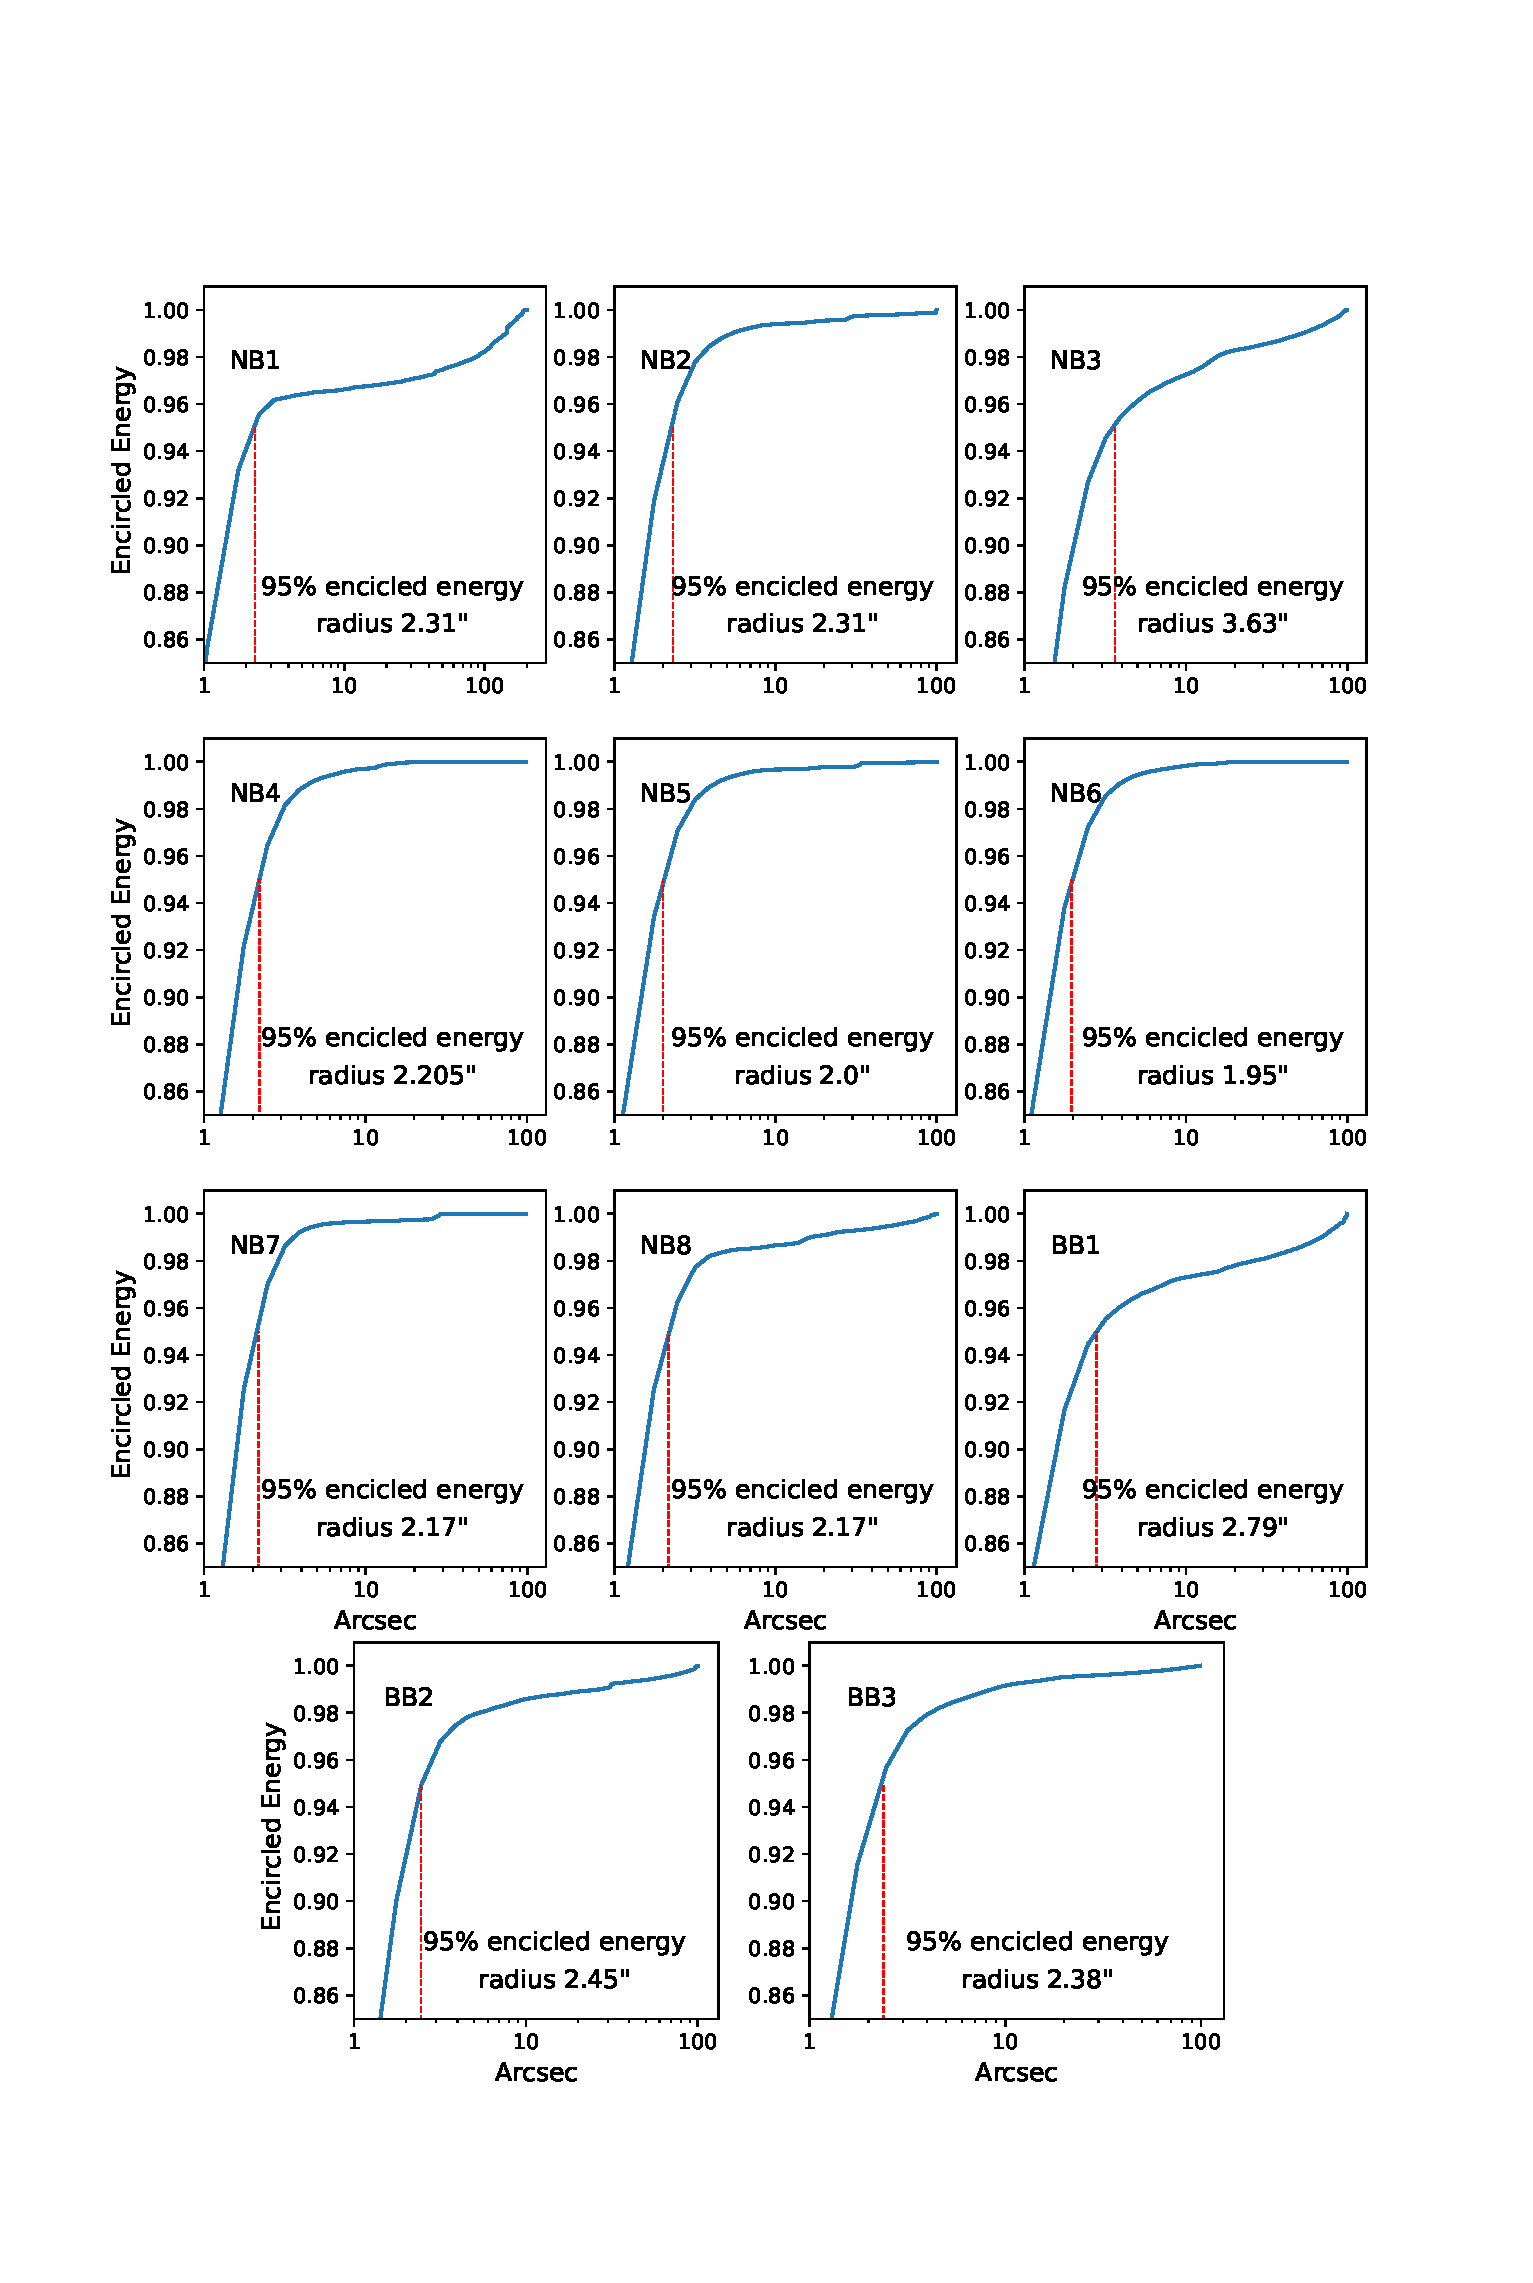
\includegraphics[trim={1.5cm 3cm 2.5cm 4cm},clip,width=0.6\textwidth]{psf_ese_2.eps}
    \caption{The encircled energy curve for the measured PSF. The 95\% encircled energy radius are marked with the vertical dashed red line. The angular scale of the 95\% encircled energy radius is also quoted in each panel for the specific filter combination.}
    \label{fig:psf_ese}
\end{figure*}
%%---------------------------%%

%%---------------------------------------------------------------
\begin{figure*}
    \begin{center}
    \resizebox{0.9\textwidth}{!}{%
        \begin{tikzpicture}[node distance=2cm]
            \node(muram)[io]{Model 3D atmospheres simulated by the radiative-MHD code MURaM};
            \node(slice)[io,right of=muram,xshift=3.5cm]{Slice the MURaM cubes and interpolate them to various $\mu$ values};
            \node(filter)[io,below of=muram,yshift=-1cm]{Use \suit~ science filter profiles accounting for all the optics on the ray path};
            \node(odf)[io,right of=filter,xshift=3.5cm]{Generate ODF tables for various filters using the MPS-ATLAS code};
            \node(rdt)[io,right of=odf,xshift=3.5cm,yshift=1.5cm]{Use ODF tables and 1D ray-atmospheres from the 3D MHD cube to carry out RT calculations using MPS-ATLAS};
            \node(int)[io,below of=rdt,yshift=-3cm]{Integrate the generated spectra for each pixel of the cube over the wavelength range of the filter profile to generate the intensity map};
            \node(conv)[io,left of=int,xshift=-4.5cm]{Convolve the total emergent intensity maps with relevant \suit~ PSF and bin to \suit~ plate scale to create mock observation};
            \draw[arrow](muram)--(slice);
            \draw[arrow](slice)--(rdt);
            \draw[arrow](filter)--(odf);
            \draw[arrow](odf)--(rdt);
            \draw[arrow](rdt)--(int);
            \draw[arrow](int)--(conv);
        \end{tikzpicture}}
        \caption{The flow chart shows the entire process of generating the simulated intensity maps, from the data cubes and characterizing the filters.}
        \label{fig:flow}
    \end{center}
\end{figure*}
%%---------------------------------------------------------------
%%---------------------------------------------------------------
\subsection{The Point Spread Function (PSF) of SUIT} \label{sec:psf}
%%-----------------------------------------------------------------

In Fig.~\ref{fig:psf_3d}, we plot the measured Point Spread Function (PSF) at the centre of the CCD for the different science filter combinations for {\suit}. The PSFs are highly peaked at the centre. The scattered light background becomes clearly visible due to the log scaling of the color bar and is more than two orders of magnitude lower than the peak.

Fig.~\ref{fig:psf_ese} shows the encircled energy curve for the measured PSFs for various filter combinations normalized to the total integral of unity. The vertical dashed lines in each plot show the radius within which 95\% of the incident light falls. For example, for the NB2 filter, 95\% of the incident light from a point source arrives within a 2.31{\arcsec} radius ($\sim$ 4.6{\arcsec} diameter) and 5\% of the light falls outside that region. Note that while the 95\% diameter is 4.6{\arcsec}, the PSF is strongly peaked. The overall diameter is considerably larger than the highly peaked part of the PSF because of the presence of a pedestal in the PSF. The pedestal is visible in all of the cases at the base of the central peak, although it is about 2 order of magnitude lower in all the cases (see Fig.~\ref{fig:psf_3d}). In some cases (e.g. NB1, BB2 etc.) a few or multiple smaller peaks apart form the pedestal are also visible. Similar radii for other filters are quoted in the corresponding panels of Fig.~\ref{fig:psf_ese}. The encircled count curves help us characterize the stray light for various filter combinations.

%%%%%%%%%%%%%%%%%%%%%%%%%%%%%%%%%%%%%%%%%%%%%%%%%%%%%%%%%%%%%%%%
\section{Forward Modeling SUIT intensity maps using MPS-ATLAS and MURaM} \label{sec:mps}
%%%%%%%%%%%%%%%%%%%%%%%%%%%%%%%%%%%%%%%%%%%%%%%%%%%%%%%%%%%%%%%%

One of the essential steps of characterizing the science filters was to conduct a thorough throughput modeling for the concerned filter combinations. However, quantifying the effects of the wavelength response of the optical components and the PSF on the spatially resolved observations, as well as the contrast variation, requires detailed modeling with resolved simulations of the Sun's surface. For this purpose, we use the MPS-ATLAS code. It is an updated version of the well established ATLAS9 \citep{atlas9} code that can efficiently generate Opacity Distribution Functions (ODFs), model atmospheres, and calculate emergent spectra in local thermodynamic equilibrium (LTE) for a given wavelength range by solving radiative transfer (RT) equation in plane parallel geometry using the assumptions of local-thermodynamic-equilibrium (LTE).

%%%%%%%%%%%%%%%%%%%%%%
\begin{wrapfigure}{l}{0.45\textwidth}
    \centering
    \includegraphics[width=.4\textwidth]{mps.pdf}
        \caption{Forward modeled intensity maps at various $\mu$ values for BB2 filter of SUIT.}
    \label{fig:flux_maps}
\end{wrapfigure}
%%%%%%%%%%%%%%%%%%%%%%

We use 3D MHD model atmospheres simulated by \cite{rempel20} and 1.5D RT with MPS-ATLAS \citep[see e.g.,][for details]{anusha21} with measured filter profiles of {\suit}, to calculate the emergent intensity. The 3D MHD simulation employs a symmetric lower boundary condition for the magnetic field and a variety of initial magnetic field configurations to create small-scale variations and various levels of magnetization. The RT equation is solved using the method of ODFs, accounting for both continuum and line opacities within the concerned wavelength range. This takes into account both continuum and line opacity within the concerned wavelength range. Accurately accounting for the line opacity is one of the major challenges in synthesizing spectra over a broad wavelength range. In the ODFs method, the opacity is sorted without the information of the corresponding wavelength within small intervals of wavelengths known as bins. The geometric mean of the sorted opacity values for multiple sub intervals within a given wavelength bin is pre-tabulated over atmospheric parameters such as temperature, pressure and micro-turbulent velocities. During RT calculations, opacity is then interpolated for the required grid parameters of the atmospheric model. The primary goal of the ODF method is to significantly minimize the computational time required for RT calculations. This becomes particularly crucial when computing emergent spectra across numerous atmospheres, such as those arising from 3D MHD simulations. 